\documentclass{standalone}
\usepackage{tikz-network}

\begin{document}
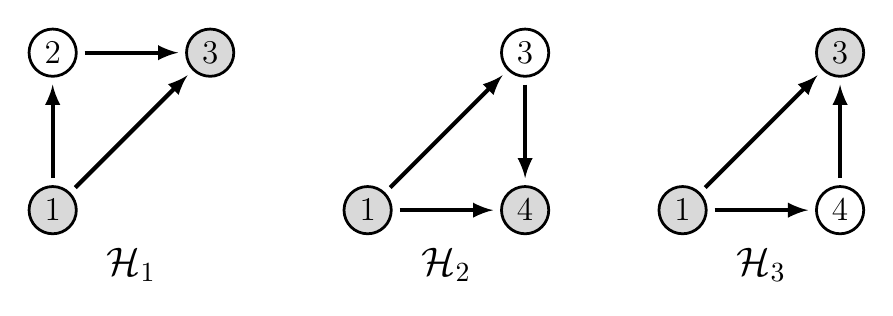
\begin{tikzpicture}

\SetVertexStyle[LineWidth=1, FillColor=black!15!white, LineColor=black, OuterSep=3, TextFont=\large]
\SetEdgeStyle[Color=black]
\SetTextStyle[TextFont=\Large]

\Vertex[label=1]{H1_1}
\Vertex[y=2,label=2,color=white]{H1_2}
\Vertex[x=2,y=2,label=3]{H1_3}
\Edge[Direct](H1_1)(H1_2)
\Edge[Direct](H1_1)(H1_3)
\Edge[Direct](H1_2)(H1_3)
\Text[x=1,y=-0.7]{$\mathcal{H}_1$}

\Vertex[x=4,label=1]{H2_1}
\Vertex[x=6,y=2,label=3,color=white]{H2_3}
\Vertex[x=6,label=4]{H2_4}
\Edge[Direct](H2_1)(H2_3)
\Edge[Direct](H2_1)(H2_4)
\Edge[Direct](H2_3)(H2_4)
\Text[x=5,y=-0.7]{$\mathcal{H}_2$}

\Vertex[x=8,label=1]{H3_1}
\Vertex[x=10,y=2,label=3]{H3_3}
\Vertex[x=10,label=4,color=white]{H3_4}
\Edge[Direct](H3_1)(H3_3)
\Edge[Direct](H3_1)(H3_4)
\Edge[Direct](H3_4)(H3_3)
\Text[x=9,y=-0.7]{$\mathcal{H}_3$}

\end{tikzpicture}
\end{document}